\documentclass[12pt]{article}
\setlength{\columnsep}{2cm}

%\usepackage{cite} 
\usepackage[round,numbers]{natbib}
\usepackage[french]{babel}
\usepackage[utf8]{inputenc}
\usepackage{graphicx} %pour mettre des figures dans multicol avec l'environnement figure*

\usepackage[T1]{fontenc} % Use 8-bit encoding that has 256 glyphs
%\linespread{1.05} % Line spacing - Palatino needs more space between lines
%\usepackage{microtype} % Slightly tweak font spacing for aesthetics

\usepackage[hmarginratio=1:1,top=2cm, right=2cm]{geometry} % Document margins
\usepackage[textfont=it]{caption} % Custom captions under/above floats in tables or figures
\usepackage{booktabs} % Horizontal rules in tables
%\usepackage{float} % Required for tables and figures in the multi-column environment - they need to be placed in specific locations with the [H] (e.g. \begin{table}[H])
\usepackage{hyperref} % For hyperlinks in the PDF

\usepackage{bm}
\usepackage{amsfonts}
\usepackage{amsmath}
\usepackage{amssymb}
\usepackage{tabularx}

%\usepackage{titlesec} % Allows customization of titles
%\renewcommand\thesection{\Roman{section}} % Roman numerals for the sections
%\renewcommand\thesubsection{\arabic{section}.\arabic{subsection}} % Roman numerals for subsections
%\titleformat{\section}[block]{\bfseries\centering}{\thesection.}{1em}{}[{\titlerule[1.2pt]}] % Change the look of the section titles
%\titleformat{\subsection}[block]{\bfseries}{\thesubsection.}{1em}{} % Change the look of the section titles
%\renewcommand\thesubsubsection{\small{\arabic{section}.\arabic{subsection}.\arabic{subsubsection}}}
%\titleformat{\subsubsection}[block]{\bfseries}{\thesubsubsection}{0.5em}{}
%\titleformat*{\paragraph}{\vspace{-0.3cm}\small\bfseries}

\newcommand{\tbullet}{$\vcenter{\hbox{\tiny$\bullet$}}~$}

\usepackage{fancyhdr} % Headers and footers
\pagestyle{fancy} % All pages have headers and footers
\fancyhead{} % Blank out the default header
%\fancyfoot{} % Blank out the default footer
\renewcommand{\headrulewidth}{0pt} %pour enlever la ligne du header
%\fancyhead[C]{titre, date, noms...	} % Custom header text
%\fancyfoot[RO,RE]{\thepage} % Custom footer text
%\fancyfoot[LO,LE]{A. DINSENMEYER, \today}
%\renewcommand{\footrulewidth}{0.4pt} 

%modif des espacement avant et après l'environnement equation
\let\oldequation=\equation
\let\endoldequation=\endequation
\renewenvironment{equation}{\vspace{-0.2cm}\begin{oldequation}}{\vspace{-0.2cm}\end{oldequation}}
 
%agrandissement de la zone de texte
%\addtolength{\oddsidemargin}{-1cm}
%\addtolength{\evensidemargin}{-1cm}
%\addtolength{\textwidth}{2cm}
%\addtolength{\topmargin}{-0.7cm}
\addtolength{\textheight}{1cm}

\usepackage{color}
\usepackage[color=blue!20]{todonotes}
\usepackage{mathtools}

%pour écrire du pseudo code :
\usepackage{algorithm}
\usepackage{algorithmic}

\usepackage{hyperref}
\hypersetup{
     colorlinks   = true,
     citecolor    = blue!90
}

\newcommand{\dd}{\partial}
\newcommand{\ok}{ \textcolor{orange}{\bfseries \textsc ok }}


\usepackage{subcaption}
\usepackage{tabulary}
\usepackage{pgfplots} 

%pour la biblio en fin de page
\usepackage{filecontents}


%----------------------------------------------------------------------------------------
%	TITLE SECTION
%----------------------------------------------------------------------------------------

\title{ {\fontsize{14pt}{14pt}\selectfont Rapport de séminaire, ED MEGA par Alice Dinsenmeyer} \\[1cm]
\fontsize{18pt}{18pt}\selectfont\textbf{ Convection and magnetoconvection in a tangent cylinder \\ Labellisé MEGA}} % Article title

\author{
\large{presented by Alban Potherat from Coventry University}\\% Your name %\thanks{}
%\normalsize École doctorale MEGA \\ % Your institution
%\normalsize \href{mailto:john@smith.com}{john@smith.com} % Your email address
\vspace{-5mm}
}
\date{le 19/01/18}

%----------------------------------------------------------------------------------------

\begin{document}
\maketitle
A. Potherat reports experiments built from scratch during K. Aujogue thesis. 

\section{Motivations}
 This work contributes to understand how the Earth sustains a magnetic field. We know this magnetic field results from the motion of a conducting fluid, located in a layer between the hot inner seed and the rocky mantel. The aim of this experimental work is thus to model the motion of this fluid, and to see the influence of the magnetic field and the rotation of the Earth on it. \\

Theoritically, rotation and magnetic field induce extra-terms in Navier-Stokes and energy equation. Consequently, if the magnetic field is weak, wavelength is driven by the rotation (viscosity), but if we increase the magnetic field to a certain point, wavelength suddenly increases, giving fat vortices.

\section{Experimental work}
The objective is to visualize flow patterns, in conditions that are close to those of the Earth (the Earth rotates very fast, if we look at the ratio viscosity/Coriolis force). In order to use optical measurement methods (PIV), they used sulphuric acid, which is transparent and has high electrical conductivity. But as this fluid is less conducting than liquids metals, the magnetic field has to be of the order of 10 Tesla. So this experiments faces multiple challenges : 
\begin{itemize}
        \item High magnetic field :
        \begin{itemize}
        		\item moving part must be ceramic, plastic, glass... (non-metallic)
        		\item no camera (PIV)
        		\item acquisition system must be above the magnet
	\end{itemize}
	\item Sulphuric acid : use chemically resistant materials and safety procedures.
\end{itemize}
The setup is given by figure~\ref{setup}.


\section{Results}
Results are compared without and with magnetic field (the later work is in progress).\\
Special modes can be observed due to symmetry breaking. These modes are very similar to those of a solid cylinder, which are wall modes caused by a lateral confinement (fluid can't escape along the horizontal plane). The confinement is related to Proudman-Taylor constraint.  In presence of the magnetic field, no structure appears in the center of the cylinder, so magnetic field reinforce lateral confinement.\\

Thermal wind is also observed resulting from a balance between Coriolis and buoyancy (heat flux).\\

No theory exists for cylinder with magnetic field, so it is a work to do.

\section{Questions}
How do you measure the wavelength ? They look at correlation on azimuthal and radial velocity.





\begin{figure}	
	\centering
	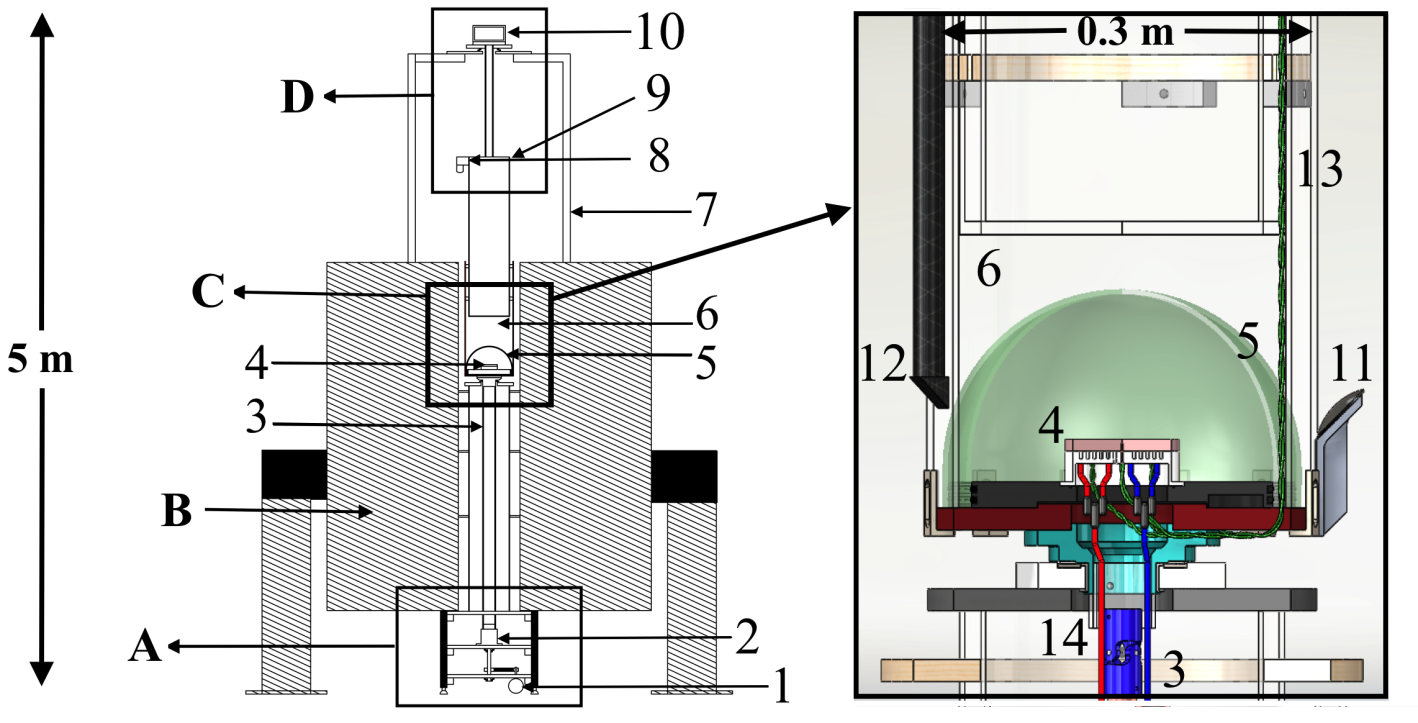
\includegraphics[width=0.5\textwidth]{img/exp.png}\\
	\caption{Apparatus design from \cite{Aujogue2016}. \label{setup} }
\end{figure}

\bibliographystyle{plainnat}
\bibliography{biblio}

\end{document}
